
\begin{figure}[h]        
    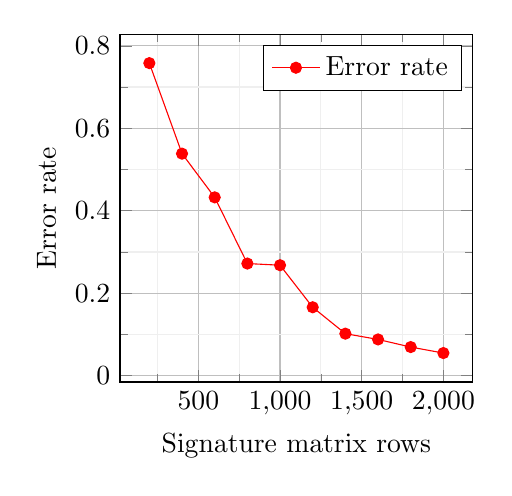
\begin{tikzpicture}
    \begin{axis}[
        xlabel=Signature matrix rows,
        ylabel=Error rate,
        height=6cm,
        width = 0.5*\textwidth,
        grid = both,
        minor tick num = 1,
        major grid style = {lightgray},
        minor grid style = {lightgray!25},
        legend cell align = {left},
        legend pos = north east
    ]
    
    \addplot[color=red,mark=*] coordinates {
    	(200, 0.758)
    	(400, 0.5385)
    	(600, 0.4325)
    	(800, 0.272)
    	(1000, 0.268)
    	(1200, 0.16600000000000004)
    	(1400, 0.10199999999999998)
    	(1600, 0.08799999999999997)
    	(1800, 0.0695)
    	(2000, 0.05500000000000005)
    };
    
    
    \legend{Error rate}
    \end{axis}
    \end{tikzpicture}
    
    \caption{\normalfont As the number of rows in the signature matrix rises, the error rate reduces.}
    \label{fig:signature_matrix_rows_error_rate}
\end{figure}
